\documentclass{article}
\usepackage[utf8]{inputenc}
\usepackage{graphicx}
\usepackage{hyperref}
\usepackage{float}

\title{Exploratory Data Analysis Report}
\author{}
\date{\today}

\begin{document}

\maketitle

\tableofcontents

\section{Exploratory Data Analysis}

\subsection{Introduction}

Before developing predictive models for customer revenue, an extensive exploratory data analysis (EDA) was conducted. The goal of this analysis was to understand the structure and quality of the data, identify potential issues such as missing values or inconsistent categories, and explore the distribution of the target variable.

The dataset consists of transaction records from 2016--2017 and a customer-level dataset containing the future revenue variable \texttt{revenue\_2018\_2019}. Transaction-level information includes product attributes, discounts, returns, and order timestamps. These transactions were aggregated to the customer level to construct behavioural features that describe purchasing patterns.

EDA focused on three main objectives:

\begin{itemize}
\item Understanding the data structure and cleaning inconsistencies
\item Exploring the distribution of key behavioural features
\item Analysing the distribution of the target variable
\end{itemize}

Understanding these aspects is important because customer revenue data is typically highly skewed and contains a large number of zero values.

\subsection{Data Cleaning and Preprocessing}

Several preprocessing steps were applied to ensure the data was consistent and suitable for modelling.

First, the transaction dataset was merged with the customer dataset using the customer identifier \texttt{cust\_id}. Date columns (\texttt{order\_date} and \texttt{pack\_date}) were parsed as datetime objects to allow time-based feature engineering.

Categorical variables were standardised by:

\begin{itemize}
\item converting text to lowercase
\item removing leading and trailing whitespace
\item standardising separators for multi-label attributes
\end{itemize}

Several product attributes such as materials, prints, and product types contain multiple labels per product. These fields were converted into lists so that they could later be encoded properly.

Rare categories can cause instability in machine learning models due to high cardinality. Therefore:

\begin{itemize}
\item rare tokens in multi-label attributes were grouped into an \texttt{other} category
\item infrequent product brands were grouped into \texttt{other\_brand}
\end{itemize}

Missing values were handled carefully:

\begin{itemize}
\item missing return information was interpreted as no return
\item missing heel information was interpreted as products without a heel
\item one observation with missing product size was removed
\end{itemize}

Finally, duplicate rows were detected and removed after temporarily converting list-based columns into tuples to allow hashing.

\subsection{Target Variable Analysis}

A key part of the exploratory analysis involved understanding the distribution of the future revenue variable \texttt{revenue\_2018\_2019}.

Figure \ref{fig:target_raw} shows the distribution of the target variable across all customers. As expected for customer lifetime value data, the distribution is heavily right-skewed: most customers generate relatively small revenue values, while a small number of customers generate very large amounts.

\begin{figure}[H]
\centering
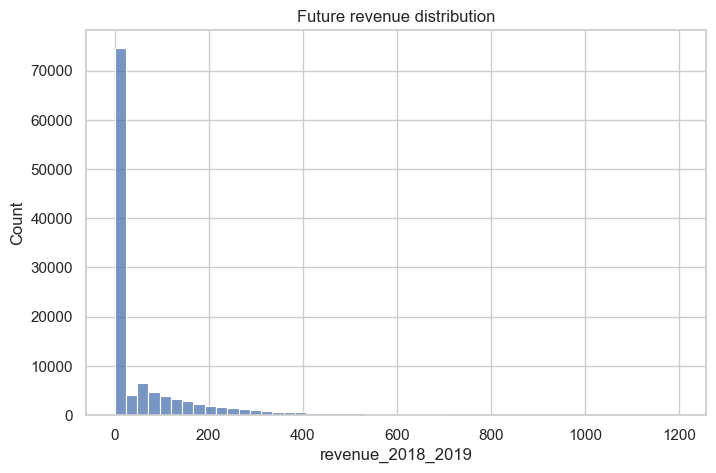
\includegraphics[width=0.7\textwidth]{eda_plots/target_distribution.png}
\caption{Distribution of future customer revenue}
\label{fig:target_raw}
\end{figure}

A common approach for handling this type of skewed distribution is to apply a logarithmic transformation. Figure \ref{fig:target_log} shows the distribution after applying a $\log(1+x)$ transformation.

\begin{figure}[H]
\centering
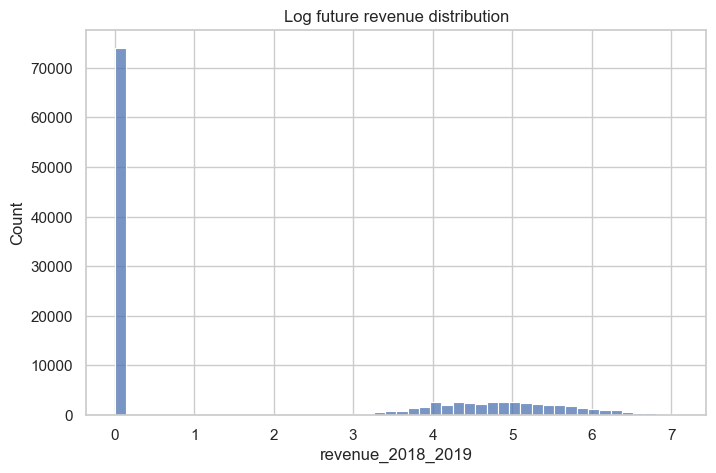
\includegraphics[width=0.7\textwidth]{eda_plots/target_log_distribution.png}
\caption{Log-transformed future revenue distribution}
\label{fig:target_log}
\end{figure}

Because a substantial fraction of customers generate zero revenue in the prediction period, the distribution was also analysed excluding zero values. The positive revenue distribution is shown in Figure \ref{fig:target_positive}.

\begin{figure}[H]
\centering
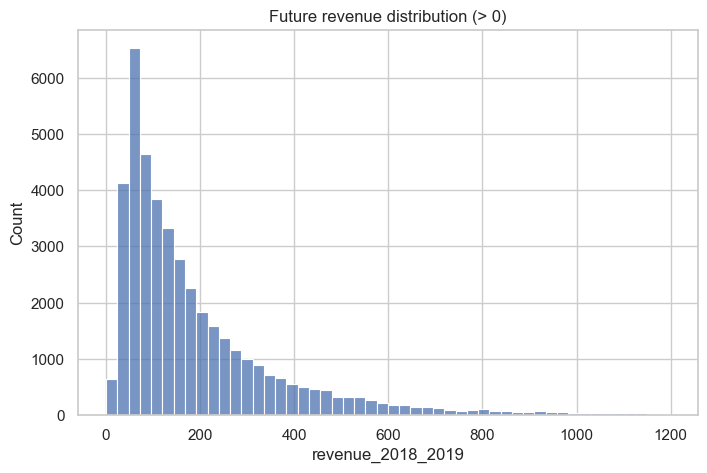
\includegraphics[width=0.7\textwidth]{eda_plots/target_distribution_no_zeros.png}
\caption{Future revenue distribution excluding zero values}
\label{fig:target_positive}
\end{figure}

The log-transformed positive revenue values are shown in Figure \ref{fig:target_log_positive}. After the transformation the distribution becomes much more symmetric.

\begin{figure}[H]
\centering
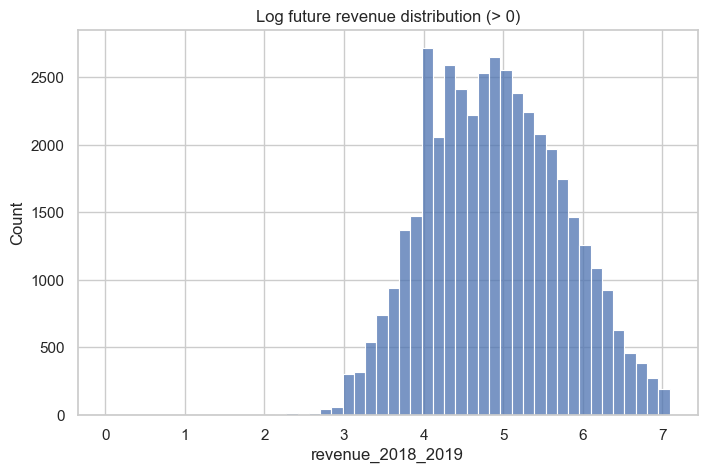
\includegraphics[width=0.7\textwidth]{eda_plots/target_log_distribution_no_zeros.png}
\caption{Log-transformed future revenue for positive values}
\label{fig:target_log_positive}
\end{figure}

To further investigate whether the log-transformed revenue approximately follows a normal distribution, a Q–Q plot was generated (Figure \ref{fig:qqplot}). The majority of observations lie close to the reference line, suggesting that the log transformation successfully stabilises the distribution.

\begin{figure}[H]
\centering
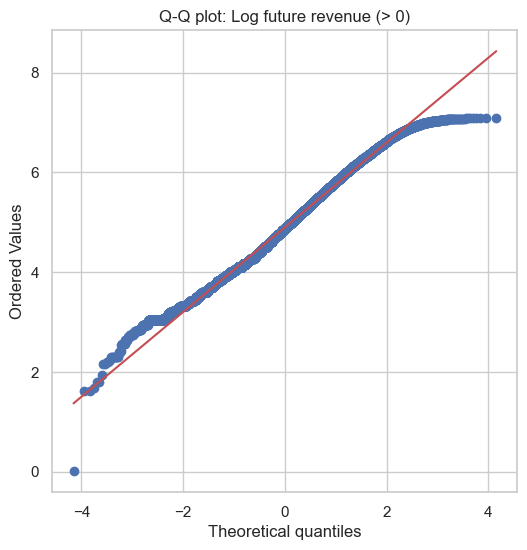
\includegraphics[width=0.6\textwidth]{eda_plots/target_log_qq_plot_no_zeros.png}
\caption{Q–Q plot of log-transformed future revenue}
\label{fig:qqplot}
\end{figure}

\subsection{Handling Outliers}

Customer revenue distributions naturally contain a small number of very large values corresponding to high-value customers. Although these observations appear as statistical outliers, they represent genuine behaviour rather than data errors.

Removing such observations purely to obtain a better fit to a theoretical log-normal distribution can negatively affect model performance. High-spending customers contain important predictive information, and excluding them would bias the model toward underestimating revenue.

Instead of removing outliers, the modelling stage benefits from using a log transformation of the target variable, which reduces skewness while retaining the information contained in high-value customers.

\subsection{Feature Distribution Analysis}

To better understand the behavioural characteristics of customers, several engineered features were examined, including:

\begin{itemize}
\item total historical spending
\item number of orders
\item recency of the last purchase
\item average order value
\item revenue generated in the last 90 days
\end{itemize}

Examples of these feature distributions are shown in Figure \ref{fig:feature_examples}.

\begin{figure}[H]
\centering
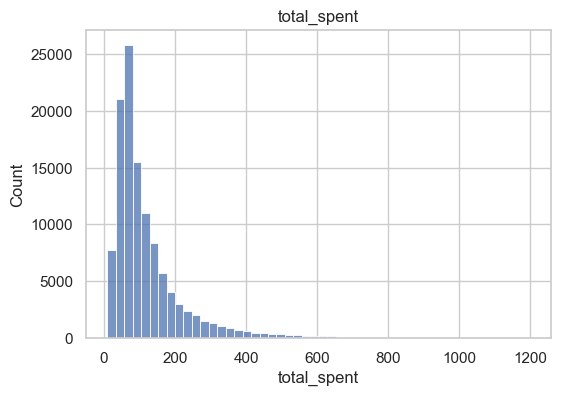
\includegraphics[width=0.45\textwidth]{eda_plots/total_spent_distribution.png}
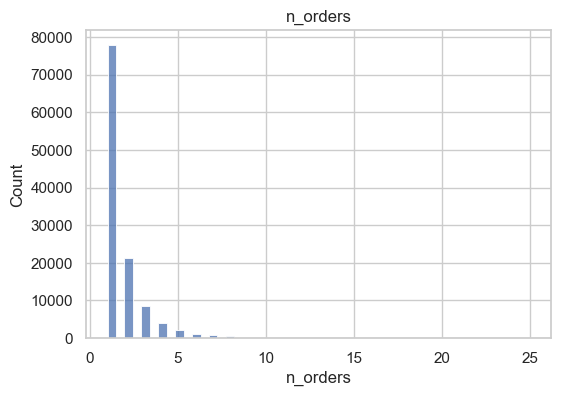
\includegraphics[width=0.45\textwidth]{eda_plots/n_orders_distribution.png}
\caption{Example distributions of behavioural features}
\label{fig:feature_examples}
\end{figure}

These distributions confirm typical patterns observed in retail data: most customers make only a few purchases, while a small fraction are highly active and generate substantially more revenue.

Understanding these patterns is essential for constructing meaningful features and selecting appropriate modelling techniques.

\end{document}
